\documentclass{article}

\usepackage{fancyhdr, graphicx}
\usepackage[table]{xcolor}

\newcommand{\stdfooter}{%
  \fancyhf{}
  \fancyhfoffset{0.5in}
  \fancyfoot[C]{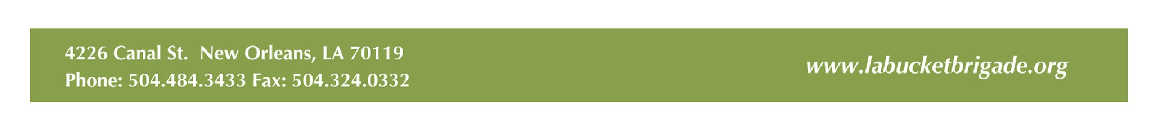
\includegraphics{footer}}
}

\fancypagestyle{plain}{\stdfooter}
\pagestyle{fancy}
\stdfooter

\setlength{\parindent}{0pt}
\setlength{\oddsidemargin}{0in}
\setlength{\textwidth}{6.5in}

\newcommand{\cubed}{$^3$}
\newcommand{\micro}{$\mu$}
\newcommand{\fc}{\cellcolor{red}}
\definecolor{salmon}{rgb}{1.0,0.8,0.7}
\newcommand{\highlightbox}[1]{\colorbox{salmon}{\parbox{\linewidth}{#1}}}

%% Some information supplied by the user:
\newcommand{\user}          {FIXME}
\newcommand{\samplename}    {FIXME}
\newcommand{\sampledate}    {FIXME}
\newcommand{\samplelocation}{FIXME}
\newcommand{\inunits}       {FIXME}
\newcommand{\outunits}      {FIXME}

\begin{document}

\title{Report}
\author{\user}
\date{}
\maketitle

\section*{Sample information}
\begin{itemize}
\item Sample identifying name:   \samplename
\item Date sample was taken:     \sampledate
\item Location sample was taken: \samplelocation
\item Report date:               \today
\item Report input units:        \inunits$^*$
\item Report output units:       \outunits$^*$
\item Report web location: http://air-toxics.dreamhosters.com/locform2.html
\end{itemize}

\section*{Unit information$^*$}
Parts per billion (ppb) describes how many weighed parts of a chemical there
are for 1 billion parts of air. For example, a recipe says to add a just a drop of
vanilla for every 100 pounds of flour. The drop of vanilla weighs hardly
anything, but it has a big effect on the cookies’ flavor. Similarly, if we measure
benzene in the air, we might find 3 “drops” of benzene for 1,000,000,000
(billion) “drops” of air. It seems like a small amount, but it is significant.
Parts per billion by volume, or ppbv, means the concentration has been figured
out in terms of how much space the molecules take up. For example, if we
make a mixture of 3 cups of vanilla and 1 billion cups of flour, then our
concentration is 3 parts volume (cups of vanilla) per billion parts volume (cups
of flour), or 3ppbv sugar in flour. When 3 volumes of benzene are in a billion
volumes of air, the concentration is 3ppbv benzene in air.
Micrograms per meters cubed (\micro g/m\cubed) describes how much of a chemical’s
weight is in a volume of air that takes up one cubic meter. Imagine an empty
box that is three feet long on both sides, and three feet tall. One meter is about
three feet long. So the box’s volume is 1 cubic meter, or 1 m 3. A microgram
(μg) is a very small weight, like that of a grain of sand. You put 3 grains of sand
into the box. The concentration of sand inside the box is 3 \micro g divided by the
volume of the box 1 m3, or 3 μg /m3. Like grains of sand, chemicals can also be
reported by weight and volume. For example, a monitor might read 5 \micro g /m\cubed
benzene, or 5 \micro g of benzene in 1 m\cubed of air.

\newpage

\includegraphics{logo}
\section*{Sample Analysis}

\highlightbox{The information below is provided to guide discussion on how
exposure to chemicals can affect you, your family, and your
community. This information is paraphrased from the ATSDR “ToxFAQs”
website available at www.atsdr.cdc.gov/sustances/index.asp.}

\subsection*{Hydrogen Sulfide}

Hydrogen sulfide occurs naturally and is also produced by human
activities. Low, long-term exposure can cause eye irritation, headache,
and fatigue. Exposure to high levels can be fatal.

\begin{tabular}{|c|c|c|}
\hline
The level in your bucket sample &                 & Comparison Level                             \\
\hline
\fc 6.27 ppb        & \fc is over 7 times         & \fc The EPA Region 6 Screening Level 0.835 ppb   \\
\hline
6.27 ppb                        & does not exceed & The Lousiana 8-hr Standard 275 ppb           \\
\hline
\end{tabular}

\subsection*{Methylene Chloride}

Exposure to methylene chloride occurs mostly from breathing
contaminated air. Breathing in large amounts of methylene chloride can
damage the central nervous system. Contact of eyes or skin with
methylene chloride can result in burns.

\begin{tabular}{|c|c|c|}
\hline
The level in your bucket sample &                   & Comparison Level                             \\
\hline
164 ppb                        & is about 48 times  & The EPA Region 6 Screening Level 3.42 ppb    \\
\hline
164 ppb                        & does not exceed    & The Lousiana 24-hr Standard 178 ppb           \\
\hline
\end{tabular}



\newpage

\includegraphics{logo}
\section*{Sample screening levels}

\highlightbox{Some government agencies have developed standards and screening levels for
toxic chemicals in the air based on health information about the chemicals.
There is no information available for some toxic chemicals. The agencies are
listed below, with a brief description of the methods used in establishing their
levels. States may not be required to adhere to national standards.}

\begin{itemize}
\item EPA Region 6 Screening Levels\newline
http://www.epa.gov/earth1r6/6pd/rcra\_c/pd-n/screen.htm\newline
These levels are based on existing studies of chemical health effects.
They levels are calculated for residential (as opposed to workplace)
exposures. They reflect the risks of exposure to a certain level of the
chemical. The levels listed as screening levels correspond to pre-
determined levels of risk from exposure: either 1 in a million cancer risk
or a "hazard quotient" of 1 for non-cancer effects, whichever
corresponds to a lower concentration. These screening levels are not
legally enforceable.

\item Louisiana Ambient Air Quality Standards\newline
http://www.deq.louisiana.gov/portal/tabid/1674/Default.aspx\newline
These levels are legally enforceable standards in Louisiana, developed
through Louisiana's regulatory process. They are found in Table 51.2 of
Title 33, Part III.
They are based on health effects information about the chemicals: the
eight-hour standard modifies occupational exposure levels to be
appropriate for residential exposures; the annual standard is based on
EPA procedures for calculating cancer risks.
\end{itemize}


\end{document}
